\documentclass[12pt,a4paper,titlepage]{article}
\usepackage[latin1]{inputenc}
\usepackage{amsmath}
\usepackage{amsfonts}
\usepackage{amssymb}
\usepackage{graphicx}
\begin{document}
	\graphicspath{{images/}{\main/images/}}
	\title{AD Tools\\User Guide}
	\author{Scott P. Morton}
	
	\maketitle
	
	\section{Get the Tool}
	The tool can be downloaded from github using open a web browser to
	\begin{quote}
	https://github.com/spmorton/AD-Tools.git
	\end{quote}
	or by issuing a git clone command from an empty directory
	\begin{quote}
	git clone https://github.com/spmorton/AD-Tools.git
	\end{quote}
	
	Keep up to date by visiting and downloading again or use 'git pull' from the cloned directory.
	
	\section{Running the Tool}
	Open a powershell console prompt and CD to the directory containing the script. Then execute the tool by typing ./AD-Tools.ps1, see Figure \ref{fig:run-prog}.
	
	\begin{figure}[h!]
		\centering
		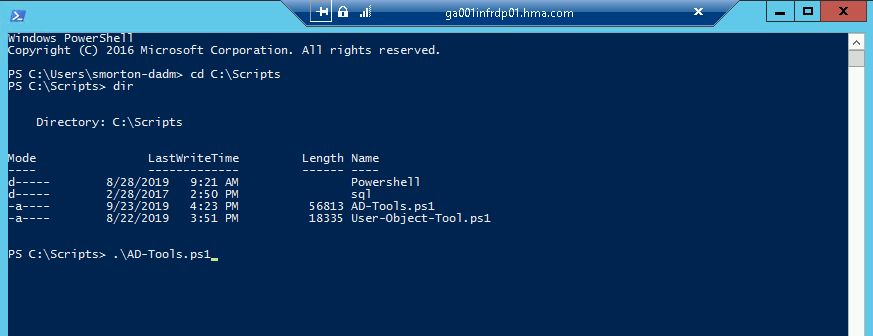
\includegraphics[width=0.9\linewidth]{run-prog}
		\caption{Open the program by typing the command displayed}
		\label{fig:run-prog}
	\end{figure}
	
	Once the tools has loaded you should be greeted witgh the following screen in Figure \ref{fig:open-prog}.
	\begin{figure}[h!]
	\centering
	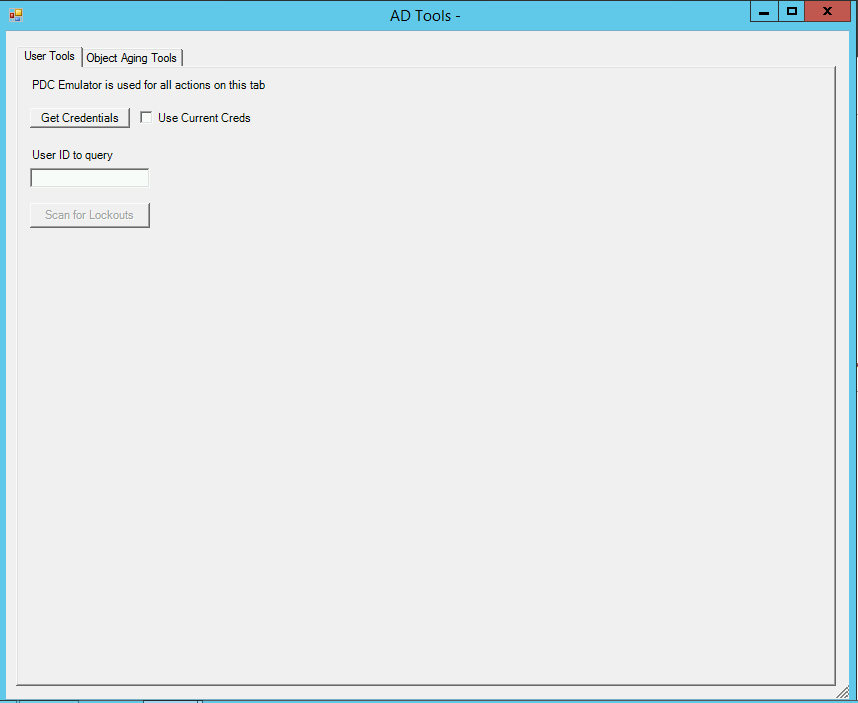
\includegraphics[width=0.9\linewidth]{open-prog}
	\caption{Initial screen displayed}
	\label{fig:open-prog}
	\end{figure}
	
	\section{Lockout Tool}
	to be completed
	
	\section{Object Aging Tools}
	Click the tab labeled 'Object aging Tools' to begin working with aged objects. For either of the selected tabs, you will need to fill in the target 'Server Name or IP address to query.' Determine your authentication type and click the 'Get Credentials'  button or check the 'Use Current Creds' box. 
	
	
	\subsection{User Object Aging}
	to be completed
	\subsection{Computer Object Aging}
	Click the 'Computer Object Aging' sub tab to begin working with the Computer Object Tool (COT). Several choices and options are available. 
	
	If you need to validate the existence of the computer, check the 'Ping Check' check box.
	
	Under filters, your choice determines how the tool functions. Choosing the defaults or changing the 'Days since LastLogonTimestamp...' drop down operates the tool in 'Disable and/or Delete' mode. Additionally, you can add the 'Enable LastModifiedDate' filter to this functional mode as well.
	
	Checking the box next to 'Search for disabled accounts with LastModfiedDate...' forces the tool into 'Delete' mode only and requires a check for 'Enable LastModifiedDate' and a selection for the number of days drop down.
	
	With your choice of filters the following procedures applies.
	
	\subsubsection{Scanning for Aged Objects to Disable/Delete}
	This scenario scans for aged object to disable. We have selected not to ping check and 60 from the drop down for 'Days since LastLogonTimestamp...' and clicked the 'Scan' button. Figure \ref{fig:cot-scanning} displays the expected screen.
	\begin{figure}[h!]
		\centering
		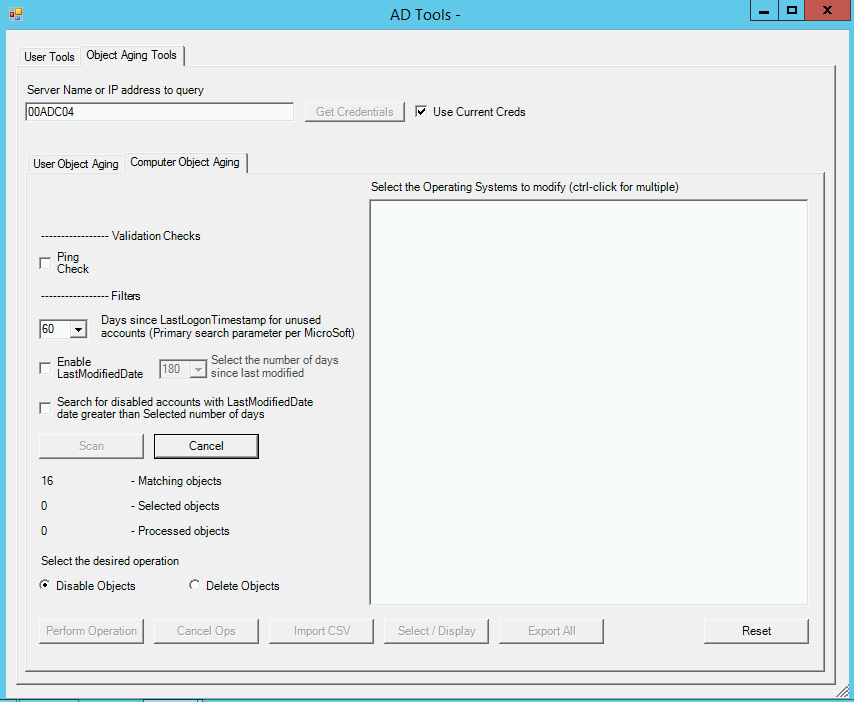
\includegraphics[width=0.9\linewidth]{images/COT-scanning}
		\caption{COT tool scanning for objects based on the selected criteria}
		\label{fig:cot-scanning}
	\end{figure}
	
	The screen will updated the 'Matching objects' counter as scanning progresses. Once the scan is complete there should be a screen similar in content to Figure \ref{fig:cot-scanning-complete}, click the 'OK' button to continue.
	
	\begin{figure}[h!]
		\centering
		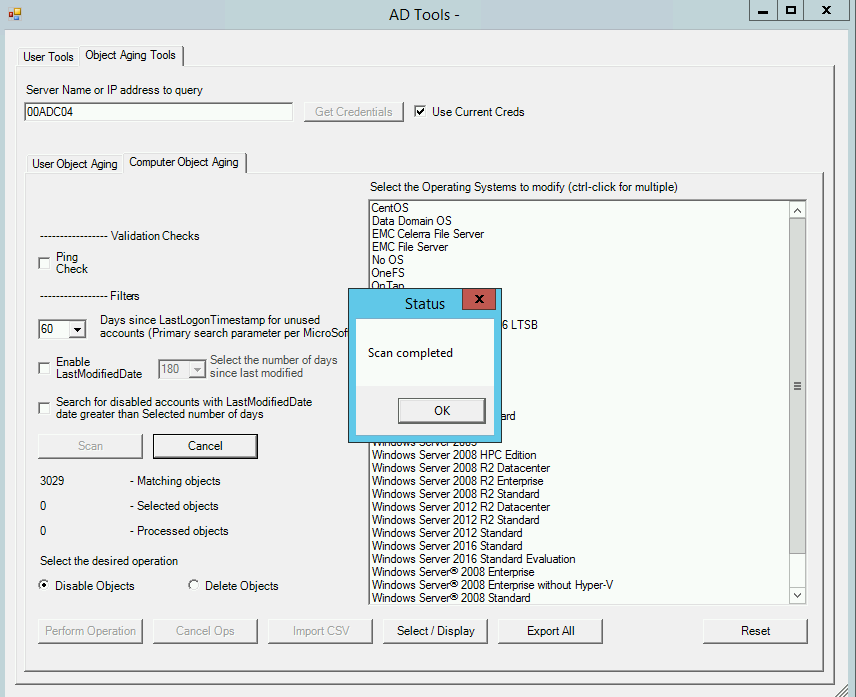
\includegraphics[width=0.9\linewidth]{images/COT-scanning-complete}
		\caption{Scan tool has completed}
		\label{fig:cot-scanning-complete}
	\end{figure}
	
	From here you have the option to export all entries by clicking the 'Export All' button below the operating system display. Optionally, and the most likely case, select the desired operating systems to act upon. in this example we are working on any Windows based systems and have selected all Windows OS' in the display as shown in Figure \ref{fig:cot-selected}.
	
	\begin{figure}[h!]
		\centering
		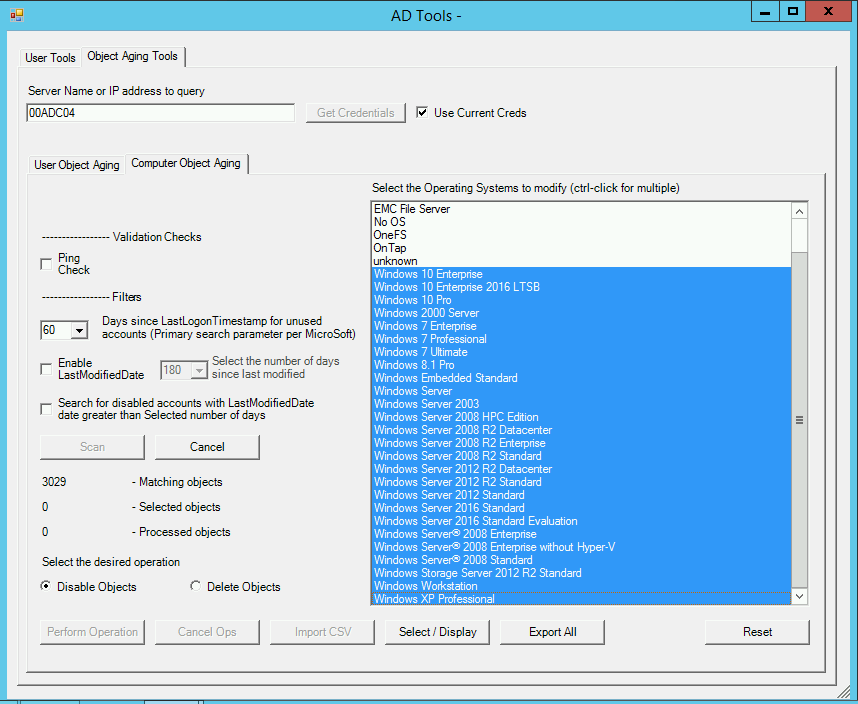
\includegraphics[width=0.7\linewidth]{images/COT-selected}
		\caption{All windows operating systems have been selected}
		\label{fig:cot-selected}
	\end{figure}
	
	At this point click the 'Select/Display' button at the screen bottom to complete the selection process and give you a chance to view the data before taking any action. Figure \ref{fig:cot-grid} represents a grid view of the data showing all attributes pulled for every object in the selection list.
	
	\begin{figure}[h!]
		\centering
		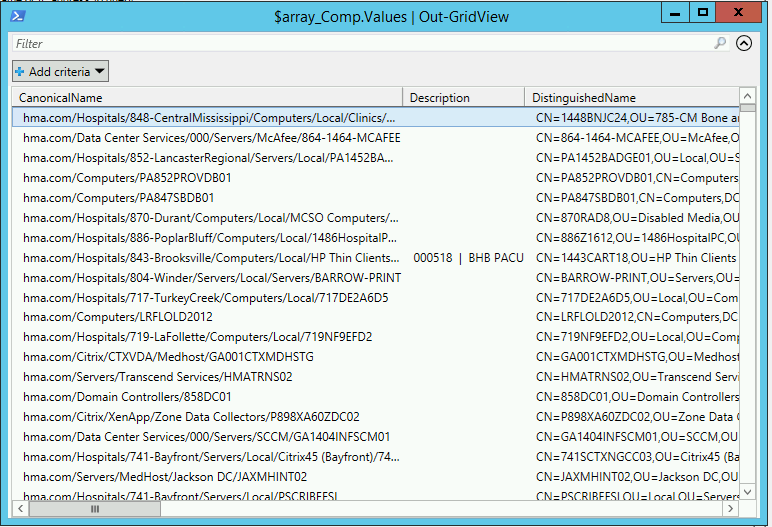
\includegraphics[width=0.9\linewidth]{images/COT-grid}
		\caption{Grid view of the selected operating systems with all attributes available.}
		\label{fig:cot-grid}
	\end{figure}
	
	The grid view can be closed at any time. To save the data for later use, click the 'Export Selected' button.
	From here decision can be made to disable or delete the selected computer objects or return to perform an operation later as described in the next section.
	
	\subsubsection{Importing From a CSV File}
	To import a CSV file, open the program as previously described and return to the 'Computer Object Aging' tab. Clcik the 'Import CSV' button at the bottom to open a file dialog and selct your previously saved data that was generated by this tool.
	
	The operating systems text box will be populated with all the OS' contained in your previous export. You will need to select and display all the OS' to act upon as previously described. At this point a decision is required as to the desired action, check the radio button of your choice and click 'Perform Operation'  at the screen bottom.
\end{document}